% !TEX TS-program = xelatex
% !TEX encoding = UTF-8 Unicode

% Example of the Memoir class, an alternative to the default LaTeX classes such as article and book, with many added features built into the class itself.

%\documentclass[12pt,a4paper]{memoir} % for a long document
\documentclass[11pt,article,twoside,openany,danish,extrafontsizes]{memoir} % for a short document
%\quarkmarks
\AtBeginDocument{\addtocontents{toc}{\protect\thispagestyle{indflytterpjece}}}

% Don't forget to read the Memoir manual: memman.pdf

\usepackage{kpfonts}

\usepackage{fontspec} % Font selection for XeLaTeX; see fontspec.pdf for documentation
\defaultfontfeatures{Mapping=tex-text} % to support TeX conventions like ``---''
\usepackage{xunicode} % Unicode support for LaTeX character names (accents, European chars, etc)
\usepackage{xltxtra} % Extra customizations for XeLaTeX

% \setmainfont{Minion Pro} % set the main body font (\textrm), assumes Charis SIL is installed
% \setsansfont{DIN 30640 Std Neuzeit Grotesk Light} % Eller: \setsansfont{DIN 30640 Std}
%\setsansfont{Akzidenz-Grotesk BQ Medium}
%\setmonofont{Deja Vu Mono}

%%% Examples of Memoir customization
%%% enable, disable or adjust these as desired

%%% PAGE DIMENSIONS
%\setstocksize{297mm}{210mm}
\setstocksize{210mm}{148mm}
%\setstocksize{216mm}{154mm}
\settrimmedsize{210mm}{148mm}{*}
%\settrims{43,5mm}{31mm}
%\settrims{3mm}{3mm}
\setlrmarginsandblock{1.5cm}{2cm}{*}
\setulmarginsandblock{1.5cm}{2cm}{*}

\checkandfixthelayout
% This is from memman.pdf



%%% PAGESTYLE
\makepagestyle{indflytterpjece}
	\makeevenhead{indflytterpjece}{}{}{}
	\makeoddhead{indflytterpjece}{}{}{}
	\makeevenfoot{indflytterpjece}{\sffamily \color{SG-roed}{\thepage}}{}{}
	\makeoddfoot{indflytterpjece}{}{}{\sffamily \color{SG-roed}{\thepage}}

\makepagestyle{kapitel}
	\makeevenhead{kapitel}{}{}{}
	\makeoddhead{kapitel}{}{}{}
	\makeevenfoot{kapitel}{}{\sffamily \color{SG-dark}{\thepage}}{}
	\makeoddfoot{kapitel}{}{\sffamily \color{SG-dark}{\thepage}}{}

\pagestyle{indflytterpjece}




%%% CHAPTERS
\renewcommand{\chaptitlefont}{\Large\sffamily\bfseries\color{SG-roed}} % set sans serif chapter title font
\renewcommand{\chapnumfont}{\Large\sffamily\bfseries\color{SG-roed}} % set sans serif chapter number font

%%% SECTIONS
\setsecheadstyle{\large\sffamily\bfseries\raggedright\color{SG-dark}} % set sans serif section font
\setsubsecheadstyle{\sffamily\raggedright} % set sans serif subsection font

%%% ToC
\setsecnumdepth{chapter}
\settocdepth{section}

%% END Memoir customization

%% PACKAGES
\usepackage[danish]{babel}

\usepackage[usenames,dvipsnames,table]{xcolor}
	\definecolor{SG-roed}{HTML}{820019}
	\definecolor{SG-dark}{HTML}{003509}
	\definecolor{SG-graa}{HTML}{888888}

	\definecolor{shadecolor}{HTML}{EEEEEE}

\usepackage{colortbl,multirow}
\usepackage{pdflscape}

\usepackage{pdfpages}
	%\includepdfset{noautoscale=true}
\usepackage{everyshi}
\usepackage{graphicx,ifthen,calc}
\usepackage{changepage}


\usepackage{tikz}
	\usetikzlibrary{positioning}
	\usetikzlibrary{patterns}
	\usetikzlibrary{shapes,arrows,shadows,fadings}
	\usetikzlibrary{decorations.pathreplacing}
\tikzfading[name=fade out, inner color=transparent!0,outer color=transparent!100]

\usepackage{soul}
	\sodef\soforside{}{0.85em}%
			{0em}{0em}
	\sodef\sohoved{}{0.5em}%
			{2em}{0em}

\usepackage[style=american]{csquotes}

\usepackage{url}
\urlstyle{rm}

\usepackage[colorlinks=true,linkcolor=SG-dark,urlcolor=SG-dark]{hyperref}
\usepackage{varioref}





\title{Indflytterpjece 2014}
\author{Skribenterne fra Gården}
\date{} % Delete this line to display the current date





\newcommand{\starbreak}{\fancybreak{$*$ \qquad $*$ \qquad $*$}}



%%% BEGIN DOCUMENT
\begin{document}

\begin{titlingpage}
\begin{adjustwidth}{-1.5cm}{-2cm}
\begin{center}
\begin{vplace}[0.75]



{\huge \scshape velkommen til}

\bigskip

\begin{tikzpicture}
	\draw [decorate,decoration={brace,amplitude=10pt},line width=1pt] (0,0) -- (11,0);
\end{tikzpicture}

\medskip

{\HUGE\sffamily\color{SG-roed} STUDENTERGÅRDEN}

\bigskip

\begin{tikzpicture}[rotate=180]
	\draw [decorate,decoration={brace,amplitude=10pt},line width=1pt] (0,0) -- (11,0);
\end{tikzpicture}

%\bigskip

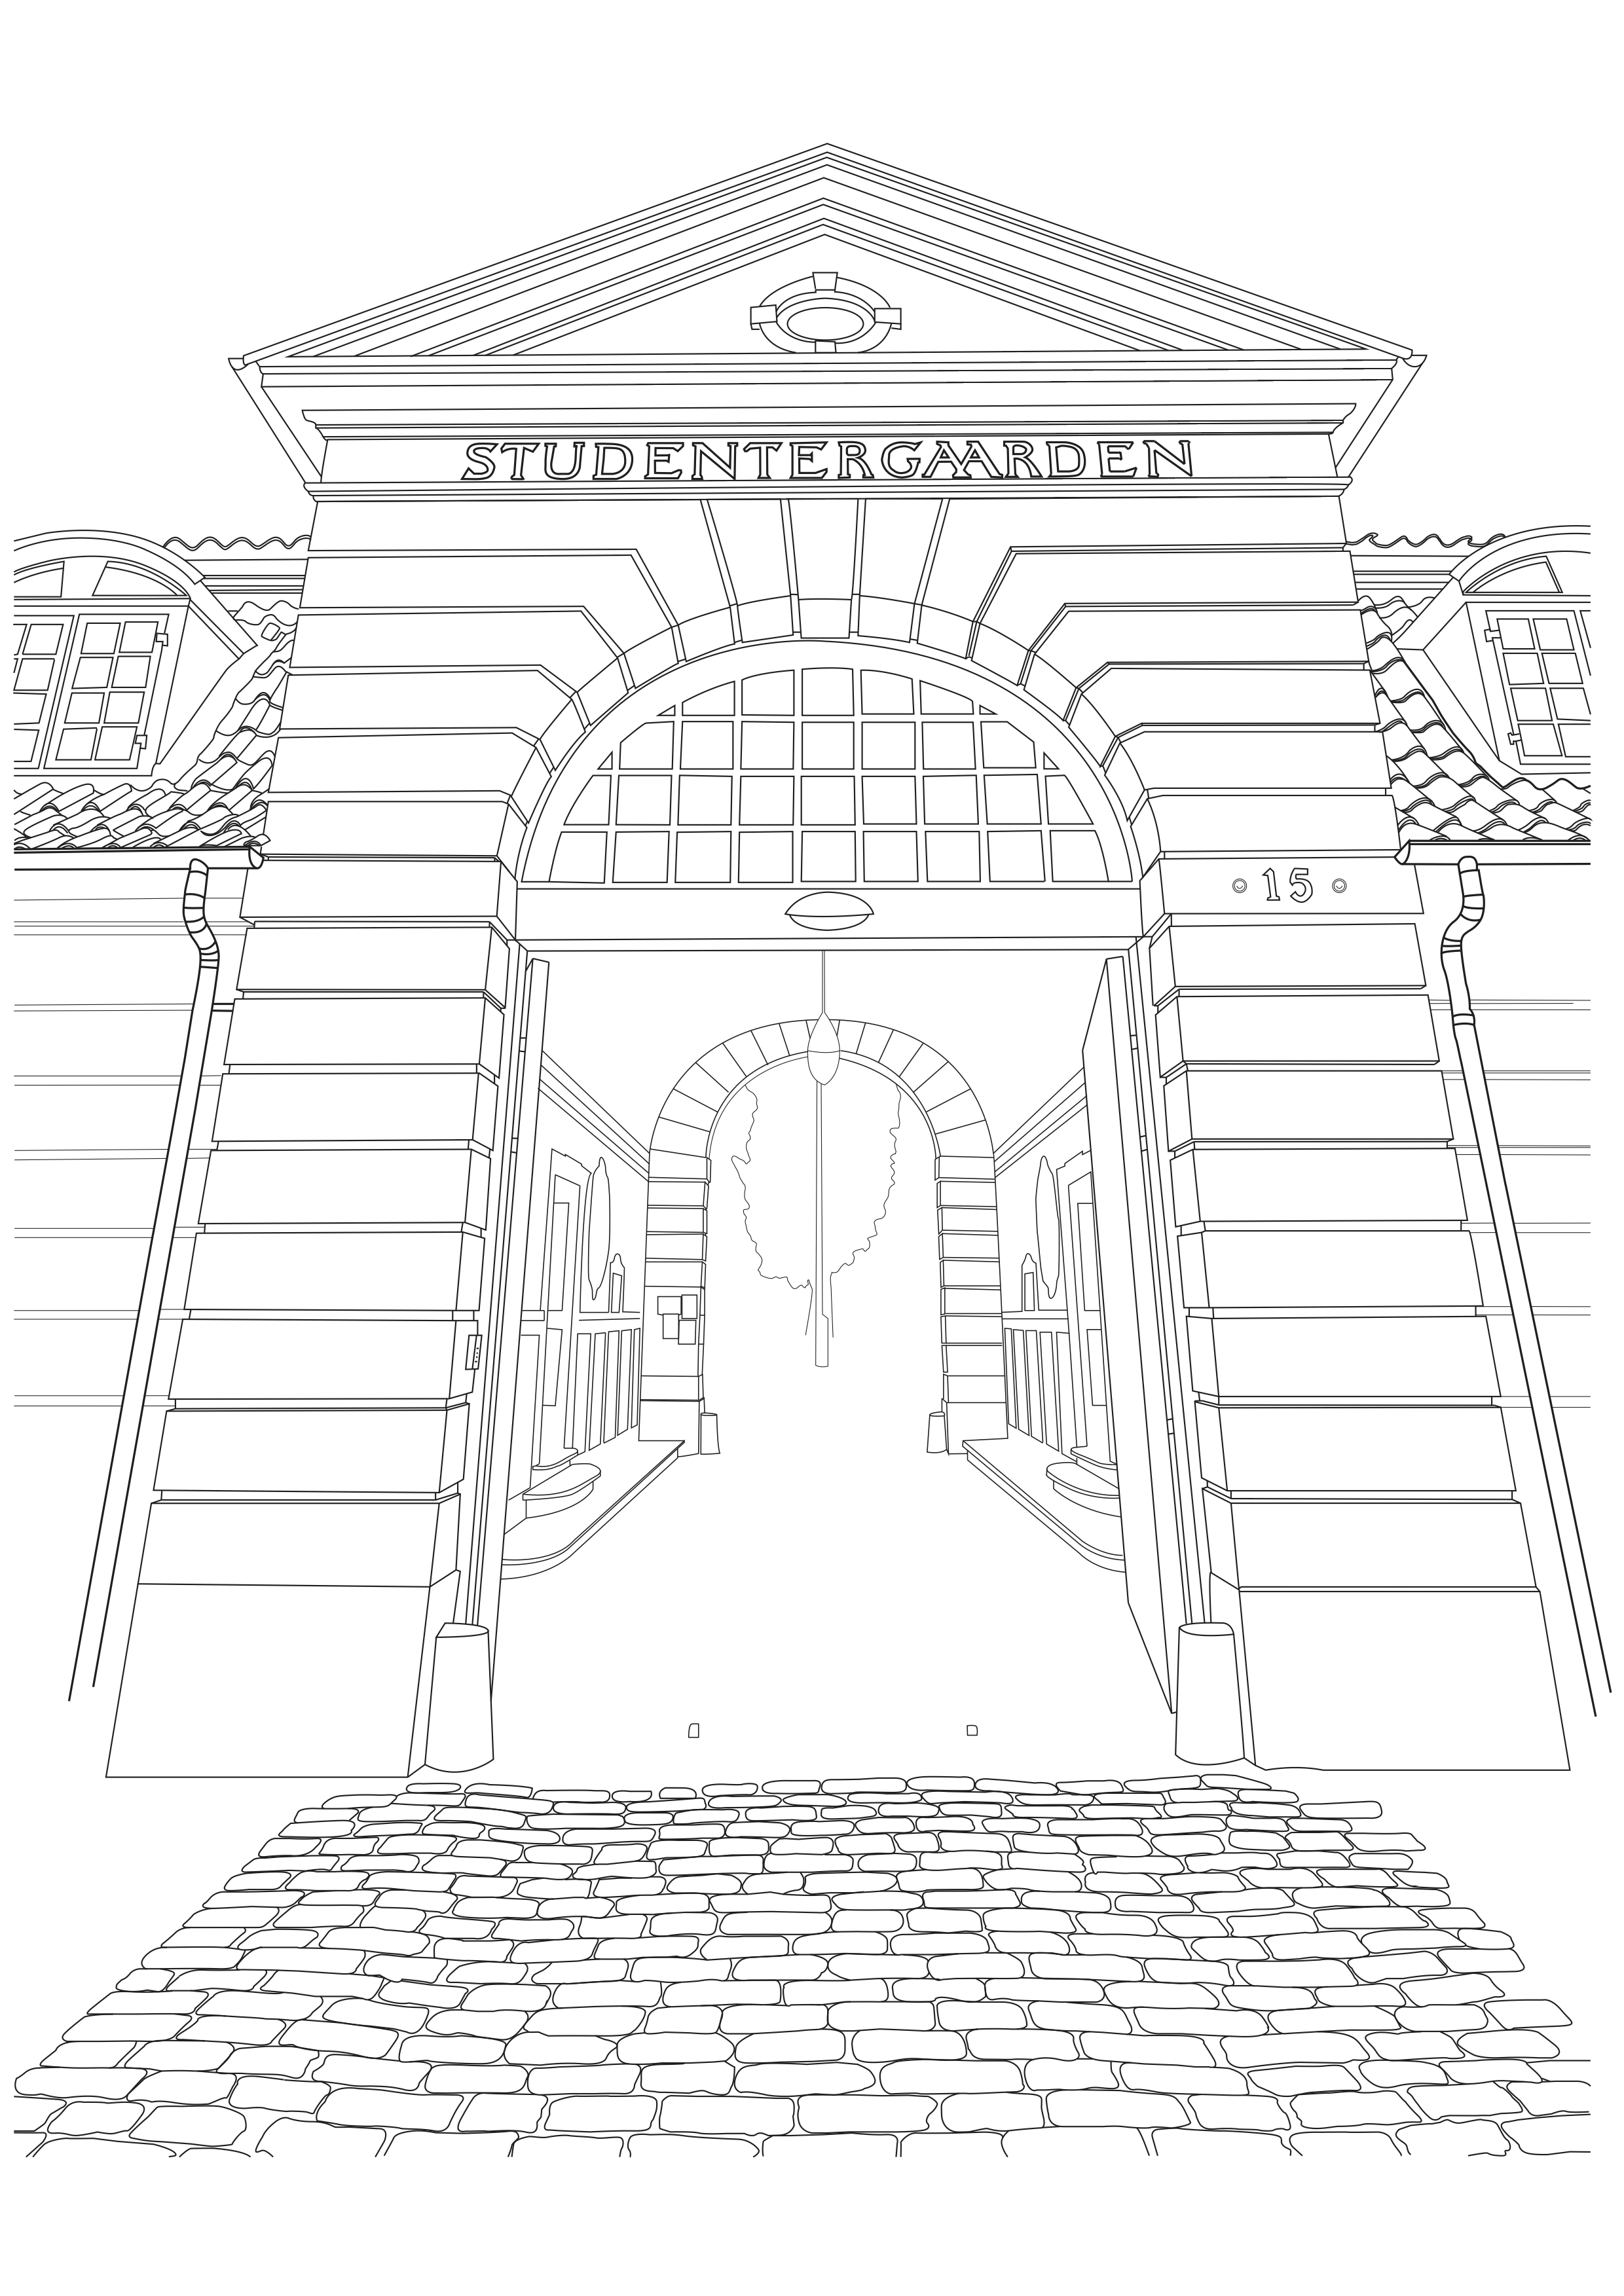
\includegraphics[width=0.75\textwidth]{fig/forside-tegning.png}

%\begin{tikzpicture}[>=triangle 45,shorten >=3pt]
%
%	\node[draw,double,circle,minimum width=2.5cm] (center) at (0,0) {GÅRD};
%
%	\node[draw,circle] (12) at (90:4cm) {FEST};
%	\node[draw,circle] (1) at (18:4cm) {LIV};
%	\node[draw,circle] (2) at (-54:4cm) {DAG};
%	\node[draw,circle] (3) at (-126:4cm) {LOFT};
%	\node[draw,circle] (4) at (-198:4cm) {LOV};
%
%	\draw[->] (center) to (12);
%	\draw[->] (center) to (1);
%	\draw[->] (center) to (2);
%	\draw[->] (center) to (3);
%	\draw[->] (center) to (4);
%
%	\draw[->] (1) to[bend left] (3);
%	\draw[->] (2) to[bend left] (4);
%	\draw[->] (3) to[bend left] (12);
%	\draw[->] (4) to[bend left] (1);
%	\draw[->] (12) to[bend left] (2);
%
%\end{tikzpicture}



\vfill


{\huge \scshape indflytterpjece}

\end{vplace}
\end{center}
\end{adjustwidth}

\clearpage

\strut\vfill

\begin{small}
\subsubsection{Tekst og redigering}
Ane Bech Andersen (Undergangen)\\
Katrine Merlach Lauritzen (Bersærk)\\
Kristina Linde Hansen (Barbar)\\
Mia Pallisgaard Hansen (Cosmos)

\subsubsection{Layout og forside}
Johan Bommelund Houby (Bersærk)\\
Søren Bang (Psykopat)

\subsubsection{Korrektur}
Anine Borger (Psykopat)\\
Anne Louise Nissen (Mellemgulvet)\\
Emil Magnus Bjerre (Pharisæer)\\
Johan Bommelund Houby (Bersærk)\\
Katrine Falcon Søby (Undergangen)
\end{small}
\end{titlingpage}




\mainmatter

\chapter*{Velkommen til Studentergården}
\textit{Kære nye gårdboer}

\medskip

\noindent
I denne pjece giver vi et indblik i livet som gårdboer. I det første kapitel fortælles om hverdagslivet, om ugens og årets gang, og om de mange forskellige udvalg. Vi giver også en lille introduktion til det, der sker i lokalområdet på den anden side af murene.


Derefter følger kapitel \vref{chap:vvv} med en beskrivelse af, hvordan du kommer på internettet, og særligt, hvordan du bruger vores intranet vvv, hvor vi har samlet de allerbedste fif, der gør livet lidt lettere. I kapitel \vref{chap:demokrati} kommer en intro til gårddemokratiet: hvordan det hele hænger sammen, og hvor du eksempelvis kan søge om penge til portvin og småkager.

Endelig følger kapitel \vref{chap:historie}, hvor du kan få et indblik i Gårdens fantastiske historie, fra den kongelige indvielse i 1923 til nutidens kamp mod stormfloder.

Allerbagest i kapitel \vref{chap:prak} finder du en oversigt over praktiske og administrative oplysninger. Brug siderne til opslag, hvis du kommer i tvivl om vaskepoletter, fremlejeregler, hvornår man må bruge Rotten og så videre.

\plainbreak{1}

Informationerne i denne pjece dækker også husordensbestemmeler, og det er et krav, at man kender til de ordensregler, vi har vedtaget. Derfor er det vigtigt, at denne pjece ikke bare bliver lagt nederst i en bunke på skrivebordet og aldrig bliver læst; som ny gårdboer skriver man under på at man har læst den, og at man vil overholde husordensbestemmelserne.

\plainbreak{1}

Velkommen til Studentergården!

\vfill

\noindent
\textit{PS. Når du ser noget i [kantede parenteser], betyder det, at du kan finde mere om emnet på Studentergårdens intranet vvv.}


\clearpage
\tableofcontents*
\clearpage

\chapter{Livet på Gården}
\label{chap:liv}

\begin{quote} \small
\enquote{Langt fremme i mindet om Studentergaarden står den hele række af herlige fester (var der seks om året eller flere?), men vigtigere var naturligvis dagliglivets lyst og nød.}

\emph{-- L.L. Hammerich, efor 1947--57}
\end{quote}

\noindent
På Tagensvej 15 bor en blandet skare. Her bor portneren Michael, eforparret Bent og Karin, rottebekæmperen Sigge og endelig de 130 gårdbrødre og -søstre. Nogle af gårdboerne har boet her i fem, seks og syv år, mens andre er helt nyindflyttede. Nogle er endnu fremlejere, mindst 11 er phiise (de senest indflyttede), og andre har for længst lært \emph{Fulbert og Beatrice} udenad.

Udefra kan det være svært at se, hvad det er, der holder beboerne sammen. Selvom nogle måske læser det samme, andre kender hinanden fra højskolen, flere har rejst sammen og en ikke ubetydelig del har fundet sammen i gårdpar, så er der ikke umiddelbart én fællesnævner, der beskriver gårdånden. Og dog -- for netop gårdånden er jo det, der samler de 130 beboere på tværs af de 11 gange. I det følgende afsnit dykker vi dybere ned i hverdagen på Studentergården.


\section{De 11 gange}
I starten kan det være ret forvirrende at holde styr på de mange gange, men bare rolig! Det skal nok komme. Du kan se gangenes placering på kortet i dette afsnit og ellers bruge de to huskeregler: CKAT og BBPP, nemlig Cosmos-Kannibal-Abort-Troglodyt for gangene i Fensmarkgadefløjen og Bersærk-Barbar-Pharisæer-Psykopat i Arresøgadefløjen. Midterfløjens Undergangen, Mellemgulvet og IVde er heldigvis til at huske.


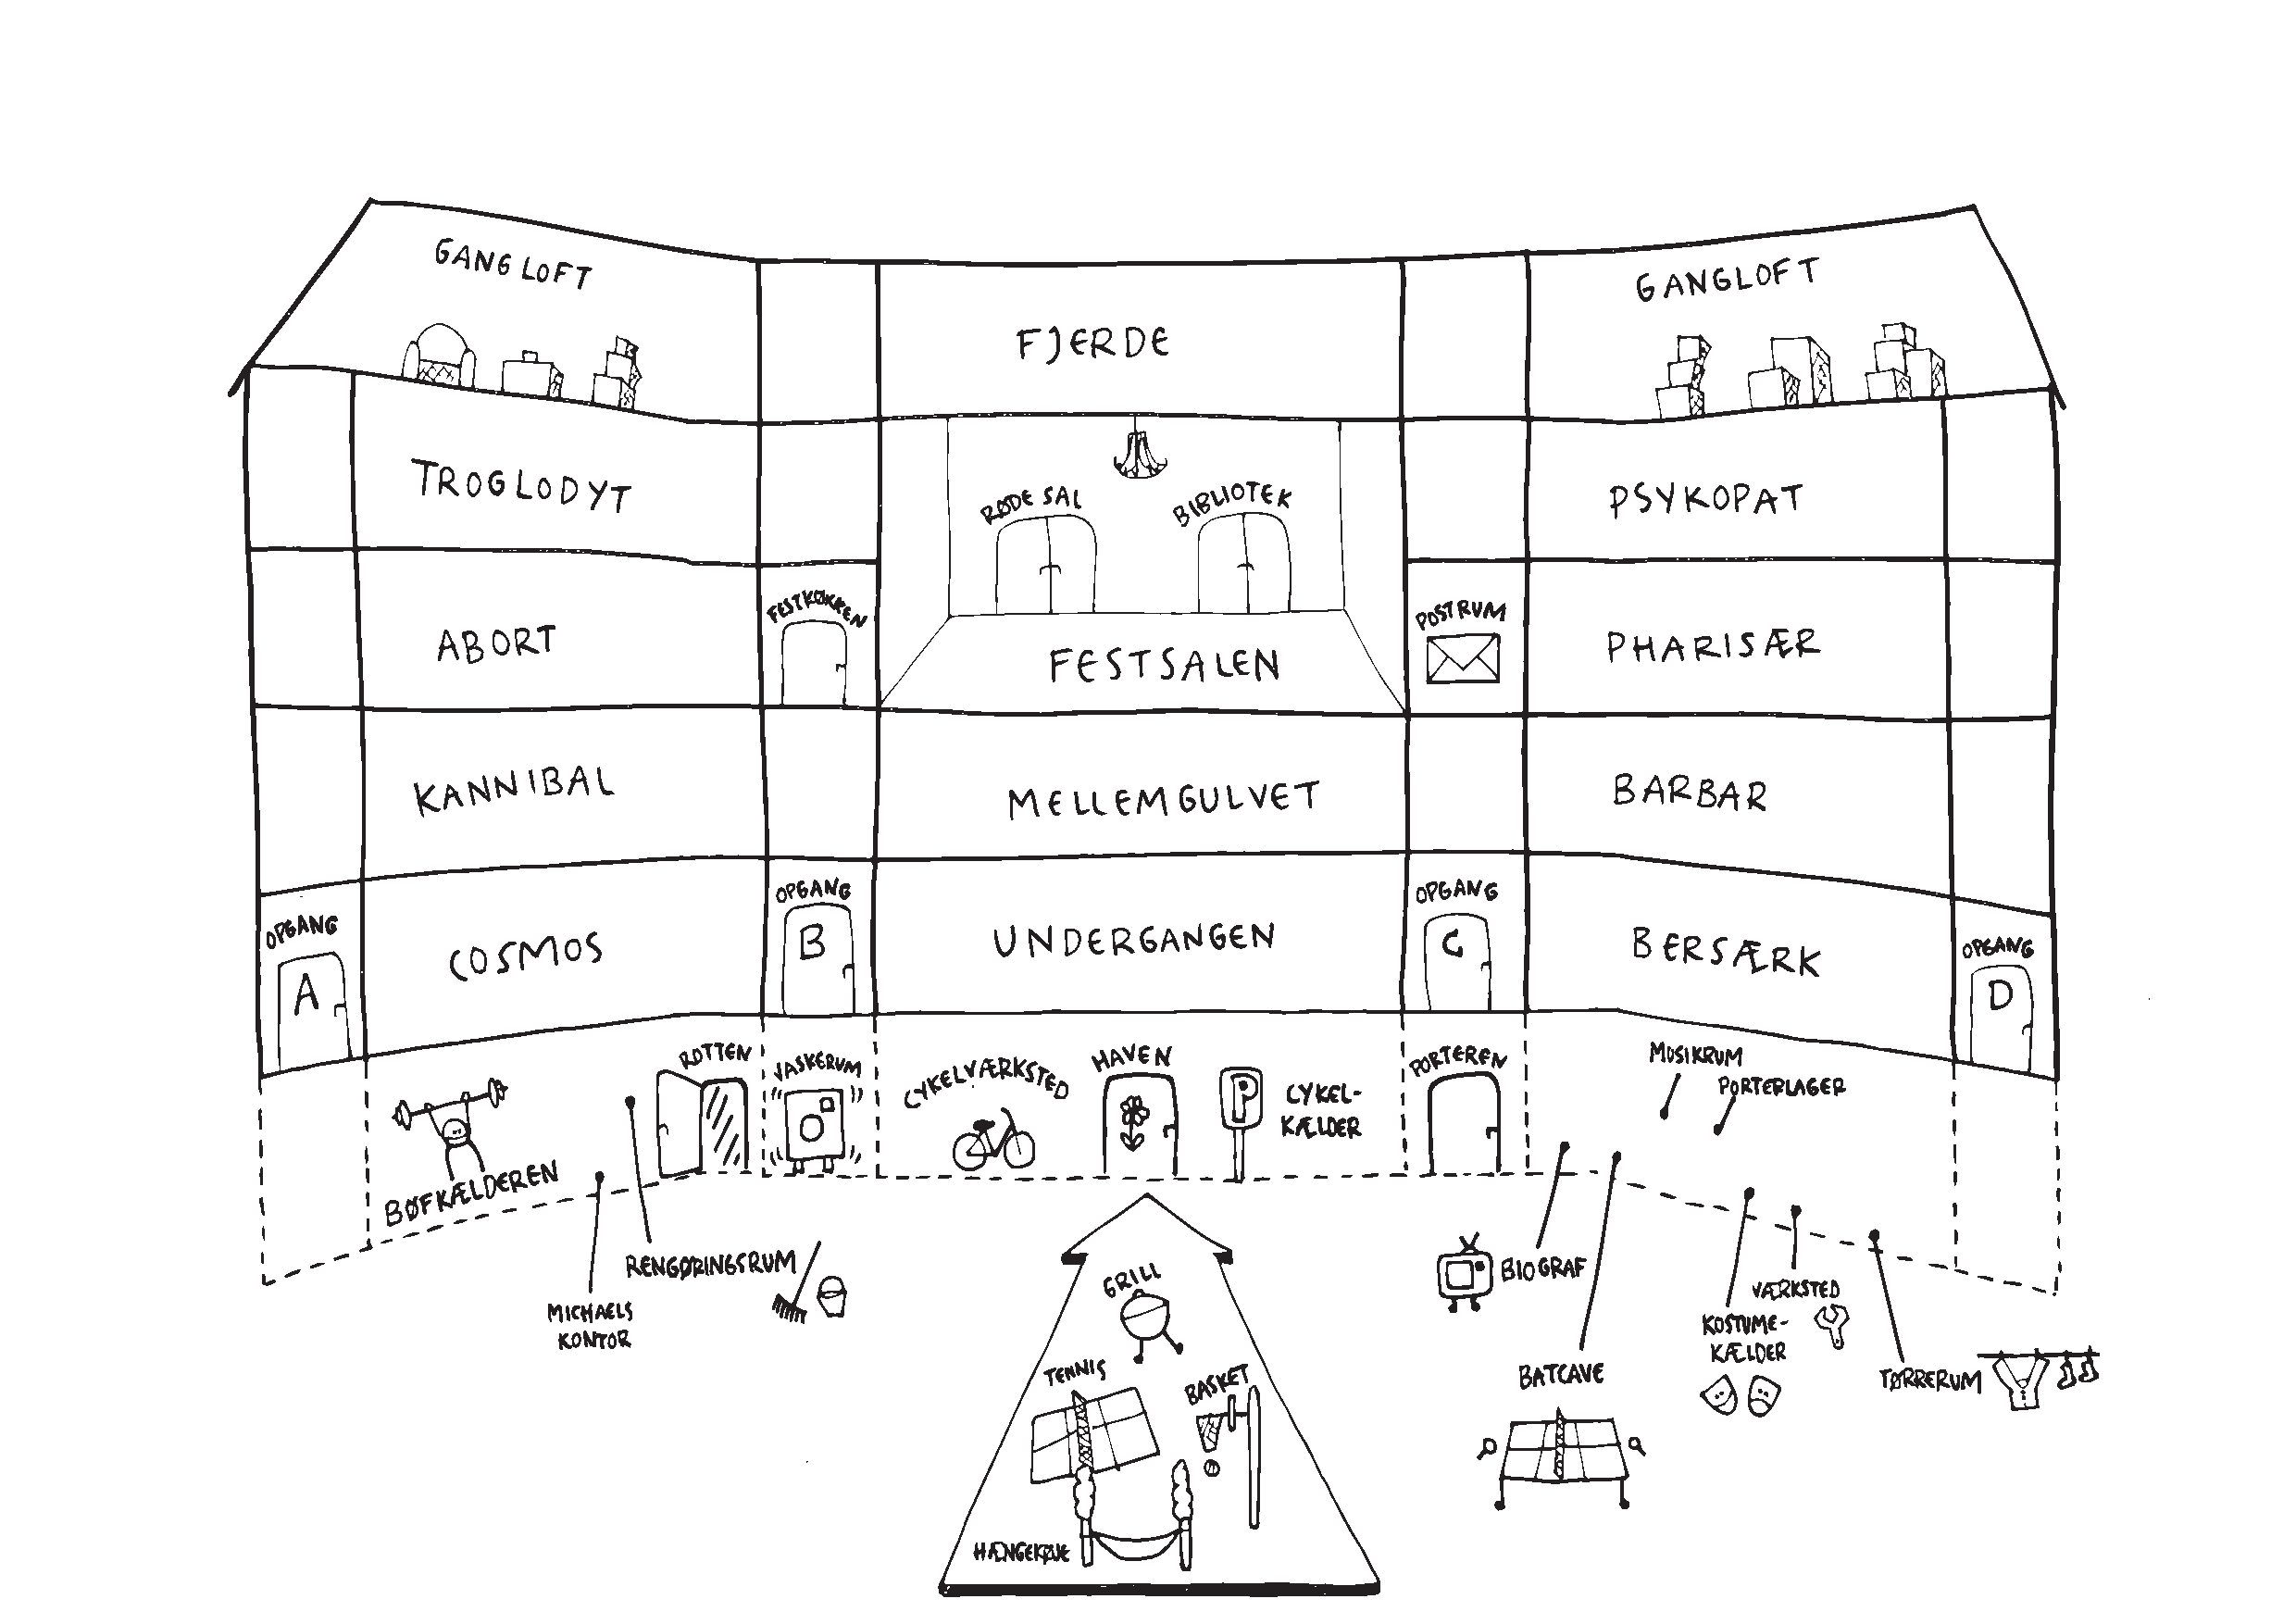
\includepdf[landscape]{fig/visuel-oversigt}


\section{Ugens og årets gang}
Studentergården emmer af hverdagsliv i løbet af året. Om sommeren kan man finde gårdboerne liggende i hængekøjer i haven, på tennisbanen til et slag tennis eller i pergolaen, hvor der grilles og inviteres til fælles madklubber på tværs af gangene. Når vejret bliver koldere, trækker gårdboerne ind i køkkenerne, Rotten og Porteren. Her hygger de sig med hjemmebag og kaffe, måske en film i biografen eller en fodboldkamp i fjernsynet. Ved nogle lejligheder finder gårdboerne deres højskolesangbøger frem og mødes til fællessang i Røde sal, eller mødes til et slag billiard i Rotten. Hverdagslivet på Studentergården sker, uden man lægger mærke til det, da det føles så naturligt og hjemligt. Har man ikke ambitioner om at lade være, kan man nemt komme til at bruge alle sine timer inden for Gårdens mure sammen med sine medkollegianere. På næste side ses et udsnit af de faste aktiviteter, som finder sted i ugens løb.

Derudover er der en række tilbagevendende hverdagsbegivenheder, som er spredt ud over året. De ligger ikke fast, men opstår, når der tages initiativ til dem. Her kan nævnes: sangaftener i Røde sal, quiz i Porteren, fredagsbar, morgenbadning, trappeløb, strikkeaftener og meget mere.

%%%% DENNE SKAL LAVES OM
%%%% JEG FIFLER
\begin{landscape}
\begin{table}[p]
\begin{center}
\begin{tabular}{|>{\sffamily}c|c|c|c|c|c|c|c|}
\hline
\textsf{TID}		&	\textsf{MANDAG}	& \textsf{TIRSDAG}	& \textsf{ONSDAG}	& \textsf{TORSDAG}	& \textsf{FREDAG}	& \textsf{LØRDAG}	& \textsf{SØNDAG} \\ \hline
\rowcolor{SG-dark!10} 8--9	& \multicolumn{2}{|c|}{Michaels kontortid}	& & \multicolumn{2}{|c|}{Michaels kontortid} & & \\ \hline
\rowcolor{SG-dark!05} 9--10	& & & & & & & \\ \hline
\rowcolor{SG-dark!10} 10--11	& & & & & & & \\ \hline
\rowcolor{SG-dark!15} 11--12	& & & & & & & \\ \hline
\rowcolor{SG-dark!20} 12--13	& & & & & & & \\ \hline
\rowcolor{SG-dark!25} 13--14	& & & & & & & \\ \hline
\rowcolor{SG-dark!30} 14--15	& & & & & & & Løverne og \\ \cline{1-7}
\rowcolor{SG-dark!35} 15--16	& & & & & & & Løvinderne \\ \cline{1-7}
\rowcolor{SG-dark!40} 16--17	& & & & & & & spiller kampe \\ \hline
\rowcolor{SG-dark!45} 17--18	& & Bents & & Bents & & & \\ \cline{1-2} \cline{4-4} \cline{6-8}
\rowcolor{SG-dark!50} 18--19	& & kontortid & & kontortid & & & \\ \hline
\rowcolor{SG-dark!55} 19--20	& & & & & & & \\ \hline
\rowcolor{SG-dark!60} 20--21	& Kor i & Porter & OnsDOK i & Porter & & & Søndagsbio \\ \cline{1-1} \cline{6-8}
\rowcolor{SG-dark!65} 21--22	& Røde sal & & biografen & & & & i biografen \\ \hline
\end{tabular}
\end{center}
%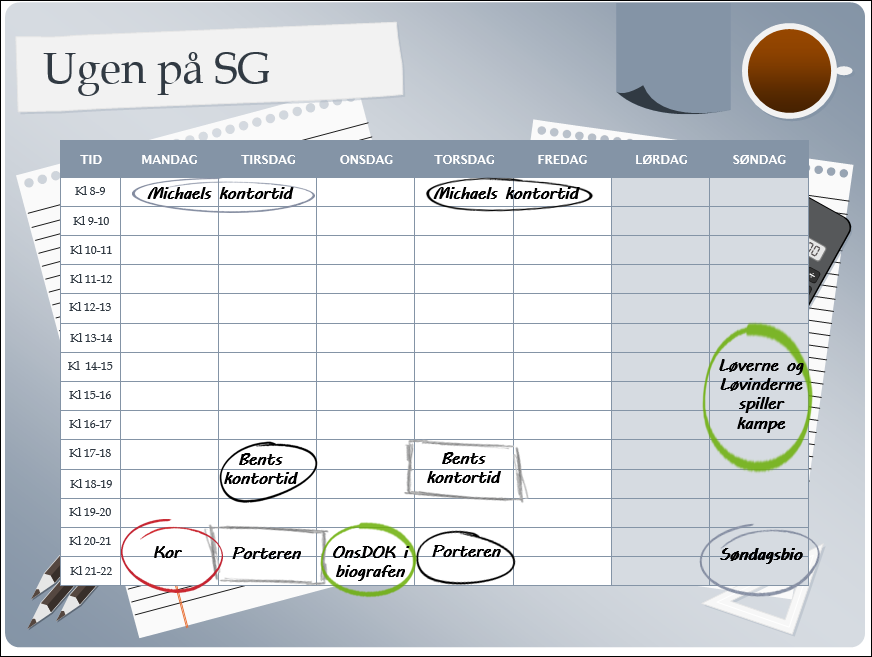
\includegraphics[height=\textwidth,angle=90]{ugekalender.png}
\end{table}
\end{landscape}


\subsection{Årlige traditioner på Gården}
Traditionerne lever i bedste velgående på Studentergården, og alle gårdboerne bidrager til, at de holdes i hævd. I løbet af året holdes fire store fester (Årsfesten, Nytårsfesten, Fastelavnsfesten og Kastanjefesten), som foregår i vores festsal, typisk med treretters middag og sang og dans til langt ud på natten. Festerne initieres af Gårdstyret og planlægges og udføres af gårdboerne selv.

Derudover rummer Studentergården også andre sjove og hyggelige traditionsrige arrangementer, som er højt værdsat blandt beboerne. Her kan bl.a. nævnes Store Bededags-arrangementet, som falder torsdag aften inden Store Bededag, hvor gårdboerne finder deres gamle studenterhuer frem og tager på fælles spadseretur på Kastellet. Efterfølgende afholdes der banko i Røde sal med varme hveder og portvin. Luciaoptoget den 13. december kan også nævnes som en af Studentergårdens traditioner. Her går en gruppe gårdboere Luciaoptog rundt på Gården, og vækker de endnu sovende gårdboere med sang. Optoget afsluttes i Festsalen, hvor der er fælles morgenmad for hele Gården og hvor koret synger et par sange.

\bigskip

\begin{shaded}
\begin{tabular}{>{\sffamily}r l}
%\toprule
Januar				& \\
Februar				& Fastelavnsfest \\
Marts				& Indflytterarrangement hos Bent og Karin \\
April				& Gårddag og forårsrengøring \\
Maj					& Gårdfejden og Store Bededags-arrangement \\
Juni				& Kastanjefest \\
Juli				& \\
August				& Det Bli’r Til Noget-festival \\
September			& SG Open og fælles arbejdsdag \\
Oktober				& Indflytterarrangement hos Bent og Karin \\
November			& Årsfest og Gårddag \\
December			& Luciaoptog og fællesmorgenmad, Nytårsfest \\
%\bottomrule
\end{tabular}
\end{shaded}

\bigskip

Ud over disse større arrangementer er der i årets løb fester og Tour de Chambre på gangene og kandidatfester i Festsalen. Endelig skal det nævnes, at der med de mange arrangementer også ind imellem er brug for en stilleweekend, hvor der ikke må holdes fester i Festsalen, og hvor man kan få ro til at hygge eller læse. Det er der typisk et par gange om måneden, så hold øje med vvv.


\section{Udvalg og udstyr}
Der er en lang række udvalg på Gården, hvor gårdboerne engagerer sig i de ting, der interesserer dem. Nogle udvalg mødes regelmæssigt, mens det for andre varierer. Kontakt endelig de udvalg, du synes er spændende, for at høre, hvad der rører sig for tiden. Du kan også selv komme på mailinglisten ved at skrive til NGM.

\subsection{Bøf \& vin} Vi prøvesmager Irmas smagsprøver og forfiner Vingårdens i forvejen herlige udvalg. %Skriv til \url{vinogboeuf@studentergaarden.dk}.





\subsection{Bøfkælderen}
Bøfudvalget har lavet den lækreste bøfkælder med træningsmaskiner og tunge vægte; nu skal den bare bruges! Udvalget står for at vedligeholde udstyret og indkøbe nyt, og der er løbende fællestræning. Hvem sagde planke? Vi elsker alle øvelser! Skriv til \url{boefkaelder@studentergaarden.dk}.

\subsection{Franskklubben}
Brie, baguettes og stumme konsonanter! Kom og bliv bedre -- alle niveauer er velkomne.

\subsection{Fundraiserne}
Vi henter penge hjem til større og mindre investeringer -- ny belægning til Gården og nye toiletter i Fensmarkgadefløjen står højt på vores liste. Skriv til \url{fundraiser@studentergaarden.dk}.

\subsection{Gaardboeren}
SG's egen avis med gøglede indslag, sladder, info fra udvalgene og uddrag fra Gårdens historie. %Skriv til \url{gaardboeren@studentergaarden.dk}.

\subsection{Gårdfejden}
Vær med til at arrangere Gårdens årlige olympiske lege, hvor køkkenerne dyster mod hinanden i farvestrålende tights, kone-polo og grillkyllingestød. Skriv til \url{idraet@studentergaarden.dk}.



\subsection{Haveudvalget}
Krydderurter, duftende blomsterbuske, grønt græs og store træer. Haveudvalget roder og regerer i Gårdens grønne åndehul.

\noindent
Skriv til \url{haven@studentergaarden.dk}.



\subsection{Koret uden Frygt}
Fordi fællessang kultiverer glæde og fællesskabsfølelse \dots{} og fordi der er kage! Find koret i Røde sal mandag aften kl. 20.15--22.00.

\subsection{Kostumekælderen}
Kan du lide glitter, kulørte drinks, udklædningstøj og æbleskiver? Så kom med i kostumekælderen -- verden har brug for blomsterbørn!

\noindent
Skriv til \url{kostumekaelderen@studentergaarden.dk}.

\subsection{Løverne og Løvinderne}
Vær med på Gårdens herre- og kvindefodboldhold, som dyster mod byens andre kollegier i den københavnske kollegieturnering. %Skriv til Katrine (BZRK).

\subsection{Miljøudvalget}
Vi gør Gården mere miljøvenlig. Kompost, regnvandsopsamling, vindmøller? Ambitionerne er store. Vær med! Skriv til \url{miljoe@studentergaarden.dk}.

\subsection{Netudvalget}
Vi binder Gården sammen -- vvv og Octavius har brug for supernørder såvel som almindelige dødelige. %Næste projekt: Fornyelse af wikien!
Skriv til \url{netudvalg@studentergaarden.dk}.

\subsection{onsDOK}
Vi viser de sprødeste dokumentarfilm onsdage i lige uger. Alle er velkomne til at sætte en film på og til at se med.

\noindent
Skriv til \url{onsdok@studentergaarden.dk}

\subsection{Porterdirektionen}
Porteren er Gårdens mødested og café. Her kan du købe øl, slik og friskristet kaffe. Porteren har åbent tirsdag og torsdag kl. 20.15--22. Hvis du har lyst til at stå i Porteren -- være \emph{kommis} -- skal du skrive til kommisdirektøren som du finder på [PorterDirektører] i wikien.

\subsection{Rotten}
\enquote{Studentergårdens udvalgsflagskib}, som det kaldes i folkemunde, er en dødhyggelig og lyssky institution, som mødes første mandag i hver måned for at fortælle røverhistorier og skabe bodegastemning på tværs af gangene. Der dystes gerne i dart, billard m.m., mens hård musik som Big Fat Snake og Erann DD kører på stereoen. Skriv til \url{rotten@studentergaarden.dk}.




\subsection{Speciale-klubben}
Speciale-klubben arrangerer fine foredragsarrangementer med Gårdens ny\-udklækkede kandidater.

\subsection{Tour-de-køkken}
Altid episk super-TDC, hvor køkkenerne underholder med hver deres tema. %Skriv til \url{tourdekoekken@studentergaarden.dk}.

\subsection{Trappeløberne}
Vi løber ugentligt på Rigshospitalets trapper og laver evt. lidt crossfit bagefter. Alle er velkomne! Skriv til \url{idraet@studentergaarden.dk}.

\subsection{Tyskklubben}
Vi mødes hver anden uge og taler tysk (på alle niveauer) ud fra et forberedt emne og  spiser tysk bagværk. Bis dann! Find gruppen på Facebook.

\subsection{Ølbryggerne}
Vi leger med mysteriet bag ølbrygningens kunst og kombinerer det gladeligt med ølstudier (det at drikke øl) og lækker mad. Skriv til \url{brygmester@studentergaarden.dk}.


\clearpage


\chapter{Livet uden for murene}
\label{chap:udenfor}

Hvis alle disse herligheder som gården rummer en dag ikke er tilstrækkelige, er der faktisk også liv uden for Gården!

\section{Caféer og mad}
Prøv at gå ned ad Fensmarkgade, og snart kommer du forbi den hyggelige og uprætentiøse vinbar Sabotøren. Et oplagt sted, når du vil invitere hende den søde fra Cosmos ud.

Går du videre rundt om hjørnet ved Refsnæsgade, støder du ind i Berlin i Københavnerformat, caféen Wascator; en hyggelig café med spil, deres egne øl og dagens ret til overskuelige priser. På Balders Plads kan du sidde i solen og drikke kaffe fra caféen Røde Rose, som også har gratis koncerter hver måned. Er tømmermændene efter gårsdagens Åbent Hus på Abort for voldsomme, kan en tur til Dilans på Jagtvej kurere det meste: snasket grillmad til ethvert behov.

Derudover er der et væld af caféer, grønthandlere og diverse takeaway-steder i Guldbergsgade, på Fælledvej, Nørrebrogade, Jagtvej og Blågårdsgade. Prøv fx [t'$\wedge$sk] på Jagtvej, som sælger frisk fisk, og lige overfor ligger bageren Brødkunsten, hvis der er behov for en onsdagssnegl eller to til kaffen på køkkenet.



\section{Barer og underholdning}
Tæt på Gården ligger Tagensborg Bodega, som altid er god for en billig bajer og tilrøgede lokaler. Trænger du til et ordentligt grin, har Vibes Apotek i Ydunsgade lattergas til salg, en god afslutning på en hård eksamensperiode.

Er du til underholdning, er der jævnligt gratis koncerter og standup på Café Mellemrummet i Ravnsborggade. På Drone på Nørrebrogade kan du give den gas fredag aften sammen med resten af undergrunden, hvis du skulle rende ind i en stilleweekend på Gården.

Hvert år i slutningen af maj afholdes Distortion; en hel dag dedikeres til Nørrebro, og man render altid ind i andre gårdboere -- husk at sætte kryds i kalenderen, hvis du er til den slags.

Er du i biografhumør, er Empire Bio på Guldbergsgade et oplagt bud. Går turen hertil, er det oplagt at tanke bland selv-slik i Palmen i Elmegade inden filmen.



\section{Grønne åndehuller og motion}
Leder du efter grønne åndehuller i nærområdet, kan Fælledparken anbefales. Assistens Kirkegård og søerne er også gode for en gåtur og en god snak. De Gamles By lige ved siden af Gården er også værd at fare vild i, her er både geder, høns og gamle huse.
På den jødiske kirkegård ved Guldbergsgade og Møllegade kan du gå dig en tur i ly for byens menneske- og trafiklarm.

Er du til skating, kan du slå dig løs i Fælledparkens nye skatepark. I Øbrohallen kan du svømme baner, og på Rigshospitalet kan du løbe trapper, til dine lår syrer til. Om sommeren kan du dyrke gratis crossfit og dans i Fælledparken.

\section{Shopping}
Er du på udkig efter nyt til garderoben til SU-venlige priser, er der i sommerhalvåret et hav af loppemarkeder i nærområdet. Der er fx loppemarkedet i Guldbergsgade (lige ved den nævnte jødiske kirkegård) hver week\-end, kæmpe månedligt søndagsloppemarked i Jægersborggade og Balders Plads. Hold dig opdateret på Facebook, eller hop på cyklen med din lige så fattige gangfælle og se, om I er heldige. Genbrugsbiksen på Fælledvej har også altid et billigt fund, og de har åbent dagligt.

Er det starten af måneden, og føler du dig ovenpå, byder området også på smarte butikker med det nyeste hipstertøj. Prøv bare at gå en tur ned ad Elmegade, så skal du nok få brugt din SU.

\plainbreak{0.5}
\fancybreak{$* \qquad * \qquad *$}
\plainbreak{0.5}

Der er faktisk ikke det, der ikke er uden for murene. Uanset hvilken vej du går eller cykler, vil du blive lokket. Men hvis det hele bliver for meget af det gode, ved du jo, hvor du bor, og hvem du kan være heldig at finde på køkkenet til backgammon og en god stempelkaffe.



\clearpage


\chapter{Internet og vvv}
\label{chap:vvv}
Studentergårdens intranet kaldes vvv og er den bedste kilde til information om ting, der sker på Studentergården. Her er tre gode tips og tricks, så du kan komme godt i gang med at bruge vvv:
\begin{enumerate}
	\item Gør vvv til din startside, så kan du let følge med i, hvad der sker.
	\item Guide til, hvordan du \enquote{klikker} dig frem til de basale ting på vvv via forsiden:

	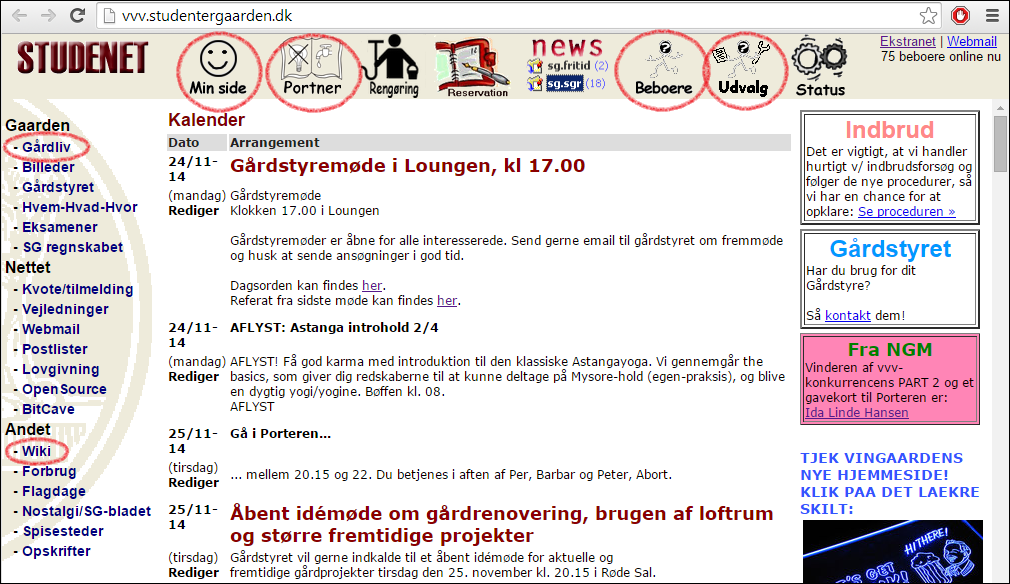
\includegraphics[width=0.8\textwidth]{fig/vvv-beskrivelse}


		\paragraph{Gårdliv:} Ud over kalenderen på forsiden er det under \enquote{Gårdliv}, du finder alle de vigtigste og praktiske informationer om Studentergården.

		\paragraph{Beboere:} Oversigt over hvem der bor på Studentergården (med navn, gang, billede, e-mail mm.)

		\paragraph{Min side:} Brug denne fane til at få adgang til vores fælles printer og køkkenregnskabet (hvis dit køkken bruger vvv’s online køkkenregnskab). Det er også her, du lægger et billede op og ændrer den mailadresse, som din studentergårdsmail videresender til.

		\paragraph{Udvalg:} Overblik over diverse udvalg og hvem du skal kontakte, hvis du har spørgsmål eller vil være med.

		\paragraph{Portner:} Kontakten til vores portner Michael. Der er kontortid alle hverdage undtagen onsdag kl. 8.00–9.00. I dette tidsrum kan du gå ned ad trappen mellem opgang A og B eller kigge efter ham i gården.

Har du ikke mulighed for at være der i åbningstiden, kan du skrive til ham her, en mulighed de fleste benytter sig af. Det er også her du får svar efter henvendelse.

Hvis Michael skal have mulighed for at planlægge sin arbejdsdag fornuftigt, skal disse to muligheder respekteres.

%Respekter venligst disse to muligheder for at komme i kontakt med din portner, da det er vejen frem, hvis han skal ha' mulighed for at planlægge sin arbejdsdag, og dermed få så meget fra hånden som muligt.

I nødsituationer (sprængte vandrør, ildebrand, krig eller stormflod) kan han kontaktes på telefonnr. 60 95 97 87.


		% Skriv her, hvis du eksempelvis har problemer med vasken, hvis der er gået en pære på gangen, eller hvis du opdager, at yderdørene ikke lukker ordentligt.

		\paragraph{Wiki:} Her findes Studentergårdens version af Google; her kan du finde svar på det meste! Prøv at kigge lidt rundt, og prøv f.eks. at søge på din gang eller på et af ovenstående ord.




	\item vvv kan godt virke gammeldags og lidt uoverskuelig, men det rummer en masse god information, så kast dig over vvv med optimisme og tålmodighed -- du får din investering tifoldigt tilbage!

	\item Husk også, at der er en helt masse grupper på Facebook for Studentergården. Du kan finde dem direkte fra vvv på [Facebook].
\end{enumerate}

\section{Internet, printer og scanner}
Studentergården har et fælles internetsystem, som man kobles op på, når man får oprettet en bruger på det fælles intranet. Spørg på din gang, hvordan du kommer online -- også med din telefon. Vejledningen findes på vvv. Der er både wifi og LAN-adgang på alle værelser og køkkener. Internettet er som udgangspunkt af god og hurtig kvalitet, men særligt vores wifi-forbindelse kan sommetider overbelastes. Derfor kan man med fordel for sig selv og sine medbeboere benytte LAN-forbindelsen, når man skal streame eller downloade store filer.

Derudover råder Studentergården over flere printere og en scanner. Alle Gårdens beboere har mulighed for at printe i sort/hvid og farver til favorable studiepriser. Selve printningen foregår som webprint fra vvv [Min side -- Webprint], hvor man uploader et eller flere dokument(er) til print. Printerne er placeret forskellige steder i huset, bl.a. i postrummet, i loungen og på Psykopats køkken. Som nyindflytter får man automatisk tildelt 10 kr. på sin printerkonto. Når disse er opbrugt, optankes printerkontoen ved at betale NGM et givent beløb, som bliver sat ind på din printkonto.

Studentergårdens scanner er til fri afbenyttelse og bor hos NGM.



\clearpage



\chapter{Kollegiets ledelse og beboerdemokrati}
\label{chap:demokrati}
Studentergårdens ledelse og beboerdemokrati er organiseret i forskellige styrende organer, der varetager hver sine opgaver. I det følgende vil Studentergårdens styrende organer kort blive præsenteret. For yderligere præciseringer af opgaver, formål og regler, kan der læses mere på vvv og i gårdloven, som er Studentergårdens beboeres vedtægter.


%%%% INDSÆT AFSNIT OM STUDENTERGÅRDENS FUNDATS

\section{Studentergårdens bestyrelse}
Studentergårdens bestyrelse består af de fem gårdstyremedlemmer og fem eksterne medlemmer valgt af Københavns Universitets bestyrelse. De eksterne medlemmer skal være heltidsbeskæftigede videnskabelige medarbejdere ved Københavns Universitet eller en anden højere læreanstalt i hovedstadsområdet eller andre personer, der nyder almen akademisk respekt. Eforen er sekretær. Bestyrelsen samles to gange årligt, typisk i forbindelse med de halvårlige ansøgningsrunder i april og november.

Bestyrelsen står for den overordnede ledelse af Studentergården; her vedtages det endelige budget og den endelige prioritering af studerende, der ønsker optagelse.

\section{Gårdstyret}
Gårdstyret består af Older, ØkonomiGårdmesteren (ØGM), OrdensGårdmesteren (OGM), NetGårdmesteren (NGM) og FundraisingGårdmesteren (FGM). Meget kort beskrevet er Gårdstyret valgt til at repræsentere og varetage gårdboernes interesser samt at realisere de beslutninger, der vedtages af Gårddagen. Desuden bestyrer Gårdstyret Studentergårdens gårdkasse, som alle gårdboere betaler til gennem den månedlige gårdskat. Gårdkassen donerer penge til sociale arrangementer eller til investeringer og inventar, der knytter sig til det sociale liv. For at få bevilget penge skal man skrive en ansøgning til \url{gaardstyre-aaben@studentergaarden.dk}. Gårdstyrets svar kan ses på vvv [News $\rightarrow$ Gårdstyre].

Men Gårdstyret varetager også mange andre opgaver. Nogle af de større faste arbejdsopgaver i løbet af året er at gennemlæse optagelsesansøgninger, drøfte budget for det næste finansår, indkalde til diverse møder af interesse for gårdboerne, herunder åbne møder for beboerne og Studentergårdens Råds møder, at hjælpe og facilitere gårdboernes initiativer og ikke mindst at holde Studentergårdens traditioner i hævd, f.eks. ved at tage initiativ til de store gårdfester. Derudover tager Gårdstyret problemer op, som opstår i det daglige liv på Studentergården.

Gårdstyremøderne er åbne, bortset fra punkter, hvor personsager indgår. Datoerne for møderne fremgår af kalenderen på vvv. Dagsordner og referater fra møderne kan findes på wikien [Kategori:Referater/GS].


\section{Studentergårdens Råd (SGR)}
Studentergårdens Råd, i daglig tale SGR, består af de fem gårdstyremedlemmer, portneren og eforen. Dette organ tager sig af den praktiske ledelse af Studentergården, f.eks. prioritering af vedligeholdelsesarbejde, udarbejdelse af det endelige budgetforslag til bestyrelsen og behandling af, hvad der ellers måtte fremkomme af forslag fra gårdboere. SGR råder over Studentergårdens økonomi, hvis indtægter er beboernes husleje. Man kan derfor ansøge SGR om penge til fast inventar på køkkenerne og andre fællesarealer, f.eks. nye brandalarmer eller service til festkøkkenet. Man ansøger ved at sende en mail til \url{sgr-aaben@studentergaarden.dk}. SRG's svar kan ses på vvv [News $\rightarrow$ SGR].

Ligesom Gårdstyret afholder SGR  månedlige møder, som er åbne for alle. Møderne fremgår af den sociale kalender på vvv, og dagsordener og referater fra møder kan ligeledes findes på wikien [Kategori:Referater/SGR].



\section{Gårddagen}
Gårddagen er gårdboernes generalforsamling og højeste myndighed. Gårddagen samles to gange årligt, i november og april, og her kan man blandt andet stille op og blive valgt til Gårdstyret. Ud over de store poster er der også andre poster på valg, f.eks. flagmand, rottemand og symaskineansvarlig. Gårddagen er stedet, hvor man diskuterer de store linjer i Studentergårdens tilværelse. Tidligere diskussionspunkter har bl.a. været reguleringen af antallet og omfanget af fester eller afstemning om hønsehus i haven.


\clearpage


\section{Organisationsdiagram}
\begin{center}
\begin{tikzpicture}[>=triangle 45] \sffamily

\node[draw,text width=60mm,align=center] (beboere) at (0,0) {\textcolor{SG-roed}{Studentergårdens beboere} \\ \smallskip

{\footnotesize 130 kollegianere, 11 køkkener}
};


\node[draw,text width=60mm,align=center] (gaarddagen) at (-2,-2.25) {\textcolor{SG-roed}{Gårddagen} \\ \smallskip

{\footnotesize Studentergården halvårlige generalforsamling}
};

\node[draw,text width=50mm,align=center,anchor=north,minimum height=3.5cm] (tillidsposter) at (-3,-4) {\textcolor{SG-roed}{Tillidsposter valgt af Gårddagen} \\ \smallskip

{\footnotesize fx flagkvinde, idrætsmand, sangbogsansvarlig, bøfkældermand og gårdkasserevisor}
};



\node[draw,text width=50mm,align=center,anchor=north,minimum height=3.5cm] (udvalg) at (3,-4) {\textcolor{SG-roed}{Åbne udvalg og frivillige initiativer} \\ \smallskip

{\footnotesize fx Porterdirektionen, fodboldholdene, miljøudvalget og haveudvalget}
};




\draw (-2,-10.5) circle [x radius= 4cm, y radius=2cm];
\draw (2,-10.5) circle [x radius= 4cm, y radius=2cm];

\node[text width=35mm,align=center] (gs) at (0,-10.5) {\textcolor{SG-roed}{Gårdstyret} \\ \smallskip

{\footnotesize Older, ØGM, FGM, OGM og NGM}
};



\node[text width=35mm,align=center] (bestyrelse) at (-3.4,-10.5) {\textcolor{SG-roed}{Studentergårdens bestyrelse} \\ \bigskip

{\footnotesize 5 eksterne bestyrelsesmedlemmer}
};


\node[text width=35mm,align=center] (sgr) at (3.6,-10.5) {\textcolor{SG-roed}{Studentergårdens råd (SGR)} \\ \bigskip

{\footnotesize Eforen og portneren}
};


\draw[->] (-1,-0.61) to (-1,-1.4);
\draw[->] (2,-0.61) to (2,-4);
\draw[->] (-2,-3.09) to (-2,-4);
\draw[->,shorten >=1cm] (0,-3.09) to (gs);

%\node[draw,text width=34mm,align=center,minimum height=5.2cm] (pragma) [right=of praesta] {
%\textbf{Pragmatikeren} \\ \medskip
%Arbejdet betragtes som: \\
%Et arbejde \\ \smallskip
%Formål med arbejdet: \\
%At udføre godt arbejde
%};


\end{tikzpicture}

\vfill
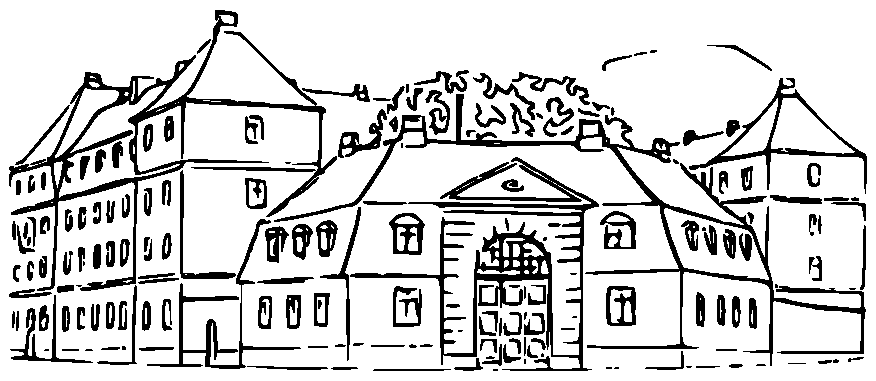
\includegraphics[width=0.6\textwidth]{fig/gaarden-tegning}

\end{center}


%%%%% NÅET HERTIL!

\clearpage


\chapter{Historien om Studentergården}
\label{chap:historie}
Studentergården blev indviet i 1923, hvor 110 gårdbrødre flyttede ind på et øde område uden for byvoldene. Siden er der sket meget ude i verden, og selvom livet inden for murene plejer at gå forholdsvis uagtet, hvad der sker udenfor, er der til tider blevet sat aftryk på livet på Gården.

I tidens løb har blandt andet Verdenskrigen og studenteroprøret sat sig deres spor, men også økonomiske hensyn og storkapitaler har præget Gårdens indre og ydre. Her følger en kort oversigt over Gårdens historie.

Bliver du bidt af historien, kan du finde jubilæumsskrifter på biblioteket, besøge Bent til en snak i hans kontortid, eller -- hvis du er rigtig heldig -- få lov at gå med ham i arkivet ved siden af Batcave.

\section{Indvielsen og Den Ny Regens}
Studentergården blev oprindeligt tænkt som \enquote{Den Ny Regens} og skulle opføres ved Regensens 300-års-jubilæum i 1923. Blandt de fire gamle kollegier i Indre København havde særligt Valkendorfs Kollegium meget plads, og den oprindelige tanke var derfor, at man ville rive kollegiet ned og i stedet opføre en større bolig med plads til 100 studerende på grunden. Der var dog en del modstand -- særligt fra Valkendorfbeboernes side -- og det endte med, at den tomme grund på Tagensvej blev givet som gave af Københavns Kommune. På det tidspunkt lå både Københavns Universitet og Den Polytekniske Højskole inden for voldene, og på Nørrebro var der endnu god plads -- og desuden gik sporvognen lige til døren.

Hovedkræfterne bag det nye kollegium var professor og læge Thorkild Rovsing, den første bestyrelsesformand, der også har lagt navn til Rovsingsgade længere ude på Nørrebro, universitetssekretær Povel Fønss og Gårdens første efor, professor Erik Arup. De to sidstnævnte fik bolig på Studentergården: Fønss i portbygningen, og Arup på det, der i dag er Undergangen. På biblioteket hænger der endnu portrætter af de tre. Da Universitetet stod kongen nær, var Kong Christian d. 10. såmænd også inviteret til indvielsen, på hvad der siden er blevet Studentergårdens fødselsdag d. 15. oktober 1923. Kongen ankom og sprang ud af sit automobil, netop som solen brød frem efter et regnskyl, og han udbrød \enquote{Jeg kommer med Tørvejr!}.
%Festlighederne varede hele dagen og sluttede med først en festmiddag i universitetskantinen i Nørregade og dernæst for lukkede døre med et punchesold i Festsalen.

De københavnske borgere bidrog på mange forskellige måder, fx er hvert værelse opkaldt efter en person eller instans, som ydede 15.000 kr. i støtte -- det var byggeprisen for at opføre et værelse. Læser man Studentergårdens fundats, der findes på den eksterne hjemmeside, kan man stadig læse, hvordan nogle værelser giver fortrinsret til vendelboere, alumner fra Birkerød Kostskole, studerende fra Rønne eller sågar til humanister fra Lunds Universitet, der nu søger optagelse på KU. En anden bidragyder var Vagn Jacobsen, søn af brygger Carl Jacobsen. Ud over flere gange 15.000 kr. gav han også de fire løver, der nu er placeret i gården, og som er afstøbninger af fire romerske kalkstensløver, der i dag findes på Ny Carlsberg Glyptotek.

Studentergårdsløverne var således en del af Gården helt fra starten og ligeledes en del af gårdboerne. For at de nyindflyttede gårdboere kunne kende hinanden, bar de nemlig de løveemblemer, der den dag i dag bliver foræret til kandidater, der flytter fra Studentergården.



\section{Indre og ydre krige}
Studentergården levede efter opførelsen sit eget liv, hvor de mest dramatiske begivenheder fandt sted inden for murene. Ikke at det var et stille liv; dykker man ned i historiebøgerne, finder man både fortællinger om \enquote{Pinsebevægelsen} i 1930, \enquote{Paladsrevolutionen} i 1938, og \enquote{Oldermandens bortførelse} i 1948.

Da krigen nåede Danmark, blev Studentergården dog berørt af besættelsen ligesom resten af landet. Universiteterne og de studerende kom i søgelyset, da de traditionelt blev anset for de største frihedskæmpere og dermed modstandsfolk. I foråret 1944 henvendte tre tyskere sig til portneren og spurgte efter gårdboeren Dragsdahl. Han var heldigvis ikke hjemme, og tyskerne tog i stedet hans skrivemaskine og en række papirer. Dragsdahl vendte ikke tilbage til Gården før efter krigen, og på det tidspunkt var hans lyse lokker blevet farvet pragtfuldt røde.

I juni 1944 var der decideret razzia på kollegiet, og en række gårdboere blev læsset på en vogn og kørt til Shellhuset, der fungerede som Gestapos københavnske hovedkvarter. Ni gårdboere tilbragte sommeren bag tremmer, mens to derefter røg til Frøslev og lejre i Tyskland. Heldigvis vendte de hjem igen efter krigen. Endelig d. 24. juni midt om natten indtræf den nok uhyggeligste nat i Gårdens historie. Her blev de tilbageværende gårdboere gjort opmærksomme på tysken, da den berygtede Brøndombande sprængte hul i muren ved Cosmos. Værelserne blev totalskadede med store huller og revner i murværket helt op til 2. sal, og flere røg på hospitalet. I dag er der indsat en mindeplade over krigen. Den hænger på indermuren ved Bersærk.



\section{Finanskrise, mados og pigelatter}
I løbet af 1950’erne, 1960’erne og helt op til 1970’erne var Studentergården præget af voldsomme økonomiske trængsler. Ikke at de studerende som sådan opdagede noget, men professoratet i bestyrelsen og bag kollegiets drift fik mange grå hår i denne tid. En del af løsningen blev at omdanne eforboligen på Undergangen til værelser og herved øge huslejebasen. Samtidig steg huslejen med en voldsom fart: I de seks år fra 1966 til 1972 steg huslejen gradvist fra 100 kr. til 300 kr. En sådan procentuel stigning vil næppe kunne gennemføres i dag.

Samtidig faldt støtten fra Finansudvalget, hele 300.000 kr., der hovedsagelig var gået til rengøring. Resultatet blev, at de studerende selv måtte finde børsterne frem. Selvom det kan virke som en kortere og forbigående periode her i bagklogskabens lys, havde flere af bestyrelsesmedlemmerne deres tvivl om, hvorvidt Studentergården overhovedet ville komme til at opleve sin egen 100-års fødselsdag. Som Anders Ølgaard for eksempel skriver i 50-års-jubilæumsskriftet i 1973:
\begin{quote} \small
\enquote{På den basis kan man vist roligt se frem til et 75 års jubilæum, men om vi vil holde 100 års jubilæum på Tagensvej, er jeg stærkt i tvivl om. [\dots] Man må imidlertid ikke glemme, at det er meget svært at forbedre bade- og toiletforhold etc. væsentligt, sådan som bygningen er indrettet. Samtidigt vil den være velegnet til overtagelse som kontorbygning, f.eks. af universitetet. Så mon der ikke kan være grund til at gætte på, at 100 års jubilæet vil blive fejret i en helt anden bygning?}
\end{quote}
I ombygningen i 1967--68 blev tekøkkenerne desuden moderniseret så meget, som det var muligt. Da det var ilde set, at mænd i starten af tyverne ikke kunne lave mad og i stedet engagerede køkkendamer, måtte gårdboerne som så mange andre til gryderne. Køkkenerne står i Fensmarkgadefløjen og midterlængen som dengang, mens Arresøgadefløjens køkkener og toiletter blev renoveret i 2008.

%I øvrigt bemærker Ølgaard også, at man i forbindelse med renoveringen af toiletforholdene måske kunne have indtænkt, at Gården ville blive lukket op for piger.
Gårdsøstre fik adgang i 1971 -- forholdsvis sent i forhold til stemningen i den omgivende verden.

\section{Nyere tids klimaforandringer}
Studentergården har i de sidste mange år været præget af at bevæge sig ind i en ny tid. Forskellige fonde har sponsoreret en række forbedringer, og ud over de nævnte køkkener tæller det i nyere tid et nyt tag og renoveringen af bøfkælder, bibliotek og musiklokale. Da portner Jørgen gik på pension i 2009, blev en række kælderrum frigjort fra opbevaring og blev indrettet med beboerbygget biograf, musiklokale, tørrerum og kostumekælder, ligesom Porteren flyttede fra portbygningen til kælderen under opgang C.

Nyligst er fremtidens klimaudfordringer begyndt at vise sig på Gården, og monsunlignende regnvejr har gang på gang givet oversvømmelser i kælderen og testet sammenholdet og beboernes gåpåmod. Alt imens hverdagen nu alligevel går videre som i næsten 100 år med Kastanjefest, Årsfest, vandinger, festival, kor, løvekampe, madklubber, kastelvandringer, ture til Five Star, temafester og rottebesøg.



\clearpage


\chapter{Praktiske og administrative oplysninger}
\label{chap:prak}

\section{Steder du kan bruge i dagligdagen}

\subsection{Bibliotek og læsesal -- [BiblioTeket]}
På anden sal i gårdens midterfløj finder du Gårdens læsesal, hvor du kan få ro til at studere. Derudover er her leksika og bøger til fri afbenyttelse, og så er det også her, alle tidligere gårdboeres bogudgivelser er samlet!

\subsection{Rotten, Gårdens bodega -- [Rotten]}
I kælderen ved opgang B ligger Rotten. Her er dart, billard og bordfodbold. Det er her, man kan hænge ud hele natten, og her mange efterfester finder sted. Man må ikke ryge i Rotten, og man skal huske at fjerne tomme øl og pant, men derudover er der frit slag.

\subsection{Biograf -- [BioGrafen]}
I samme kælderlokale som Porteren ligger biografen. Hver søndag kl. 20.30 sætter biografdirektørerne en film på. Se på vvv, hvilken film der er aftenens aktuelle, og kom derned i god tid -- nogle gange er man heldig, at Porteren åbner med friske forsyninger af slik og popcorn. Hver anden onsdag sætter \emph{onsDOK} en dokumentar på, og ud over de faste film kan du også selv få lov at sætte en film på, bare den slutter senest kl. 22 af hensyn til Bersærkerne ovenpå, som kan høre hvert et actionbrag.

\subsection{Bordtennis i Batcave -- [Batcave]}
I kælderen ved opgang C står Gårdens bordtennisbord. Her kan du tage en double med din nabo eller en omgang rundt-om-bordet med gangen. Titlen som bordtennisansvarlig vindes hvert år ved en nervepirrende turnering.

\subsection{Træn i Bøffen}
Bøfkælderen ligger i kælderen ved opgang A. Her kan du træne dine \emph{guns}, og der er romaskiner, vægtskiver og måtter til diverse udskejelser -- bare du husker den gode teknik, så du ikke ryger i \emph{snap city}!


\subsection{Lav store måltider i festkøkkenet -- [FestKøkkenet]}
Festkøkkenet ligger på 2. sal ved opgang B. Det anvendes til store arrangementer -- til hverdag og fest -- såsom Studentergårdens traditionelle fester, kandidatfester og lignende.


\subsection{Festsalen}
Festsalen ligger på 2. sal i midterfløjen og bruges i forbindelse med Studentergårdens traditionelle fester, kandidatfester, bryllupper og runde fødselsdage. Hvis man skal booke Festsalen til et arrangement, skal det gå gennem OGM.


\subsection{Musikrummet}
Musikrummet ligger i kælderen ved opgang C. Her er basismusikinstrumenter og en god dunst af ægte øvelokale. Man booker lokalet ved at skrive sig på tavlen uden for lokalet. Det kan bruges af alle (uanset talent) indtil kl. 22. Studentergården har også et flygel i Røde sal. Flygelet kan anvendes til at øve mandag til søndag kl. 11.30--12.30 og igen kl. 18.30--20.00. Det begrænsede tidsrum skyldes, at der, i så vid udstrækning som muligt, skal være ro i biblioteket til at læse. Vær desuden opmærksom på stilleperioder.


\subsection{Hæng ud i Porteren}
Studentergårdens egen lille købmand! Her kan du købe øl, slik og friskristet kaffe. Porteren har åbent tirsdag og torsdag fra klokken 20.15 til 22. Hvis du har lyst til at stå i porteren -- være \emph{kommis} -- skal du skrive til kommisdirektøren som du finder i wikien [PorterDirektører].


\subsection{Røde sal}
Røde sal ligger bag ved Festsalen i forlængelse af biblioteket og bruges til diverse arrangementer, fx Store Bededag. Her hænger portrætter af en række eforer samt af Gårdens grundlægger Rovsing. Røde sal inddrages ofte som dansegulv til store fester i Festsalen.


\subsection{Tennis og basket}
Studentergården besidder sin egen tennisbane (og basketnet), som ligger bag ved hovedbygningen i forlængelse af haven. I sommermånederne bruges den flittigt af gårdboerne og deres venner. I september måned kommer al sommerens sved på prøve, da Studentergårdens Tennismand indkalder til den årlige tennisturnering for Gårdens erfarne og mindre erfarne tennisspillere. Arrangementet hedder i daglig tale SG Open.

Tennisbanen er tilgængelig året rundt. Udgang til tennisbanen sker via cykelkælderen. I cykelkælderen finder du også Gårdens ketsjere og tennisbolde. Når tennissæsonen er på sit højeste, er det muligt at booke banen i et tidsrum på en time via den tavle, som hænger oven over tennisudstyret i cykelkælderen.



\subsection{Værkstedet}
I kælderen ved opgang D ligger værkstedet. Her er der boremaskiner, arbejdsborde, svejseapparat og masser af materialer, der kan bruges til alverdens projekter. Der er adgang for alle med værelsesnøglen, men værktøjet er låst inde. Den værkstedsansvarlige har nøglen hertil og findes på vvv under  [Udvalg].

\subsection{Kostumekælderen -- [KostumeKælderen]}
Kostumekælderen ligger i kælderen ved opgang C. Her er udklædning til enhver festlig lejlighed, og du må låne lige så tosset, du vil -- bare du husker at hænge det på plads efter brug.

\subsection{Vingangen}
Skal du til fest, eller har du bare lyst til at nyde et glas rødvin til aftensmaden? Ingen grund til at bevæge sig uden for murene: Studentergården har sin helt egen vingang, hvor du kan købe flasker og bag-in-a-box. Vingangen vælges årligt på Gårddagen.

\subsection{Pergolaen -- [Pergolaen]}
Pergolaen er græsstykket i gården, hvor der både er bænke og grill. Den bruges ofte til madklub, fester og andre arrangementer i sommerperioden, og når vejret tillader det. Hvis man vil bruge den til større arrangementer, kan man reservere den via [Reservation] på vvv. Hvis man vil larme eller feste efter kl. 22, skal man dog trække indenfor -- måske til Rotten?

\subsection{Haven}
Studentergården har nok Nørrebros største have og eneste private tennisbane. Her kan du bruge hængekøjen, der ligger i cykelkælderen, eller benytte bænke, grill og bålplads til madklubber. Da en tredjedel af Gården har værelser ud til haven, skal man dæmpe sig kl. 22 og eventuelt trække ned i Rotten. Hvis tørretumbleren kører, er det tilladt for havegæster at slukke den.





\section{Praktiske gøremål}

\subsection{Vask}
Vaskekælderen ligger i kælderen ved opgang B. Her er to vaskemaskiner, tørretumbler og tørrerum. Man skal reservere vasketid nede i vaskerummet -- der ligger et skema, som man kan skrive sig på. Poletter til vaskemaskinen og tørretumbleren koster 15 kr. og købes på den gang, hvor vaskeriinspektøren, VIP, bor. Spørg på gangen, hvem det er.

\subsection{Tørring}
Der ligger både et tørrerum i forlængelse af vaskekælderen og et tørrerum i kælderen ved opgang D. Derudover er der en tørretumbler i vaskerummet. Når vejret er godt, kan det også anbefales at tørre tøj i haven. Der hænger tørresnore på tennisbanen.

\subsection{Post}
Postrummet ligger på 2. sal ved siden af biblioteket. Man finder sin post bag den låge med sit efternavns forbogstav. Husk at hente din post jævnligt, og tjek også det nederste rum til store pakker.

\subsection{Cykler og cykelværksted}
Under Gårdens midterfløj findes cykelkælderen og cykelværkstedet, hvor der blandt andet findes cykelværktøj, en kompressor til at pumpe din cykel og en krog, som du kan hænge din cykel op på og fikse den. Af hensyn til pladsen er det ikke tilladt at have mere end to cykler i kælderen.

\subsection{Når noget går i stykker}
Gårdens portner Michael holder til i kælderen mellem opgang A og B -- med indgang ude fra gården. Han kan hjælpe med at ordne ting på dit værelse eller på gangens køkken. Skal du bruge hans hjælp, kan du kontakte ham på vvv [Portner] i øverste fane. Derudover har han åbent værksted alle ugens dage (undtagen onsdag) fra kl. 8--9 i kælderen.

\subsection{Fødselsdag}
Studentergårdens flagmand m/k står for at hejse flaget på mærkedage, og når nogen har fødselsdag. Husk derfor at indtaste din fødselsdag på vvv i [Min side]. Du kan se andre gårdboeres fødselsdag under menuen [Andet $\rightarrow$ Flagdage].

\subsection{Print}
Se kapitel~\ref{chap:vvv} om, hvordan du kobler dig til Studentergårdens printere. Hvis alt går helt galt, kan der printes på universitetsbiblioteket KUB Nord på den anden side af gaden. Her skal man oprettes som bruger og kan tanke op; det koster 55 øre pr. side.

\subsection{Når det bliver koldt}
I løbet af de kolde måneder er Studentergården -- på trods af den hjertevarme, beboerne bidrager med -- ikke altid det varmeste sted i København rent temperaturmæssigt. Værelserne og gangene er ikke isoleret efter nutidens forskrifter og kan derfor blive meget kolde om vinteren. Med initiativ fra bl.a. miljøudvalget har vi dog gjort rigtig meget for, at værelserne og gangene bliver holdt nogenlunde varme i løbet af vinteren, og at vores varmeregnskab ikke bliver tårnhøjt. Alle vinduer på værelser og gange er derfor udstyret med forsatsruder i glas eller plexiglas, og vinduerne har gummilister i tætningerne; det hjælper alt sammen med at holde på varmen. Alle værelser har desuden en radiator, der kan varme i de kolde måneder. Brug den med omhu, og luft ikke ud på dit værelse, mens radiatoren er tændt. Er gummilisterne blevet møre og skal udskiftes, kan du skifte dem selv; der ligger friske lister i rengøringsrummet. Hvis der er mere galt -- fx hvis radiatoren er i udu -- kan du kontakte Portneren på vvv [Portner].

\subsection{Brand! -- [BrandProcedure]}
Studentergården har heldigvis aldrig oplevet brand (7-9-13!), men vi tager selvfølgelig vores brandforholdsregler. Alle værelser og køkkener skal være udstyret med røgalarmer. Disse er lokale og bipper, hvis den opsnapper røg. Derudover er Studentergården udstyret med et centralt alarmsystem, som manuelt slås til i tilfælde af brand. Disse alarmer kan høres på alle gange og på alle værelser. Når alarmen går, skal alle beboere mødes i gården, hvilket fremgår nærmere af procedurerne for brand, som du kan læse om på vvv. Der afholdes årlige brandøvelser.

\subsection{Indbrud}
Når man opdager et indbrudsforsøg, er det vigtigt, at man først noterer sig omfanget af indbruddet. Dette kan gøres meget enkelt ved at notere
%\begin{enumerate}
	1)~hvor indbruddet har fundet sted,
	2)~indbruddets omfang og
	3)~hvornår man observerede indbruddet.
%\end{enumerate}
Dernæst viderebringes disse tre informationer til OGM-suppleanten via \url{ogm@studentergaarden.dk}.

\subsection{Skadedyr}
På køkkenet skal du være særlig opmærksom på møl, der blandt andet lever af mel, gryn, kerner, nødder, tørret frugt med mere, og som typisk kommer ind via økologiske madvarer. Brug tætsluttende beholdere, sæt tape på huller og andre oplagte mølreder, gør hyppigt rent og kassér inficerede fødevarer.

Øget rejseaktivitet og uheldige indkøb kan desuden medføre forekomst af skadedyr på værelse. Vær opmærksom på usædvanlige forhold (kløe, småkryb mv. der kan være tegn på væggelus, lopper eller lus). Man har pligt til at anmelde den slags til portneren.

\subsection{Rengøring}
Som gårdboer har man selv den største del af ansvaret for, at Studentergården er ren og pæn. På fællesområderne såsom gangene, opgangene, toiletterne og badene kommer der et rengøringsfirma forbi på ugentlig basis. Det kræver selvfølgelig, at rengøringspersonalet kan komme til, så sørg for ikke at have mere end én måtte og ét par sko stående på gangen.

Hvert år har vi desuden forårsrengøring og arbejdsdag, hvor det hele bliver vasket ned. Rengøring af gangens køkken foregår som regel ved ugentlig turnusordning, man skiftes til på køkkenet. Denne turnusordning har forskellige navne på forskellige køkkener, f.eks. slavetjans, køkkenhelt og alf.

\subsection{Aviser}
Det er op til hver enkelt gang, hvor mange og hvilke aviser man vil holde, og disse betales over køkkenkassen. Avisspørgsmålet tages typisk op på et køkkenmøde en eller to gange årligt.

\subsection{Frysere}
Køkkenernes frysere er placeret forskellige steder på Gården. Bersærk, Barbar, Pharisæer og Psykopat har frysere placeret i et skab på gangen, IVde og Troglodyt har frysere på loftet over Troglodyt, mens Cosmos, Kannibal, Abort, UG og MG deles om tre frysere i Batcave ved opgang C. Desuden kan fryserne i kælderen også bruges til særlige lejligheder som kandidatfester og andre store fester, så længe maden fjernes efter arrangementet.

\subsection{Gangskat}
Alle gårdboere betaler et månedligt beløb til køkkenkassen. Dette går til krydderier, avis og hvad der ellers er besluttet at være fællesindkøb. Typisk er det ikke et kontant beløb der betales hver måned, men et beløb der indgår i et samlet regnskab, for eksempel via indkøb til køkkenet. Køkkenerne bestemmer selv beløbet.




\section{Husleje, værelser, anciennitet, fremleje og orlov}

\subsection{Husleje og depositum -- [Husleje]}
Den gældende huslejesats kan altid ses på vvv. Den skal betales  senest den 15. i hver måned kontant til eforen eller til
\begin{quote} \small
Reg: 3199

Konto: 7113099
\end{quote}
Det er vigtigt, at du angiver navn og værelsesnummer, og skulle man glemme at betale til tiden, er der en rykker på 100 kr. Bemærk at huslejen ikke opkræves, men er beboernes eget ansvar at indbetale månedligt på det oplyste kontonummer. Af den månedlige husleje går 20 kr. til gårdkassen, som støtter sociale arrangementer på Studentergården. Læs mere om dette i kapitel~\ref{chap:demokrati} under Gårdstyret. Depositum svarer til to måneders husleje, men gælder ikke som faktisk husleje. Det er beboernes eget ansvar, at melde indflytning samt interne flytninger til Folkeregistret.

\subsection{Indflytning}
Før indflytning vil din kommende gang tage kontakt til dig. De vil typisk invitere dig på madklub og vise dig det værelse, du kommer til at overtage. Ved indflytning udleveres tre nøgler fra udflytter. Husk at melde indflytning til Folkeregistret. Eventuelle skader og mangler ved indflytningsværelset skal meldes til portneren senest 14 dage efter indflytning.

\subsection{Udflytning og depositum -- [UdflytningsFormular]}
Senest seks uger før du flytter ud, skal du have skrevet en opsigelse til eforen. Når du flytter, skal du sørge for at aflevere dit værelse i god, pæn og ren stand til den næste indflytter. Ved fraflytning skal eventuelle malede vægge males hvide igen; der kan findes maling i rengøringsrummet. For at få dit depositum tilbage, skal du udfylde en udflytningsformular, som kan findes på vvv. Den skal underskrives af forskellige folk, blandt andre den, der overtog dit værelse, og lånekassemanden. Ved udflytning synes det fraflyttede værelse, og eventuelle skader dækkes af depositummet. Hvis ikke alle tre nøgler haves, bestilles nye hos portneren.


\subsection{Maling}
Hvis dit værelse er en smule slidt ved indflytningen, har du mulighed for at hente gratis hvid maling i rengøringsrummet i kælderen, så det igen kan blive flot og skinnende. Her er ligeledes afdækningsplast, grundrens, pensler og ruller. Vær opmærksom på, at der er både vægmaling og træmaling til paneler, vindueskarm og døren.

\subsection{Værelser og anciennitet}
Man optjener anciennitet som gårdboer -- det vil sige, at den gårdboer, der har boet på Gården længst, har førsteret til at vælge værelse på gangen. Ancienniteten flytter i princippet med på tværs af gangene, men der opfordres dog til, at man taler om det på den gang, hvor man bor.

Anciennitet tælles fra indflytningsdagen. Under orlov (se nedenfor) opnås ikke anciennitet. Fremleje (se nedenfor) giver ikke anciennitet; dette gælder såvel udlejer som fremlejer. Beboere, der kommer tilbage fra orlov eller efter fremlejes ophør, har anciennitet som før.


\subsection{Fremleje -- [FremlejeRegler]}
Som hovedregel skal fremlejere opfylde de samme krav som ansøgere, der ønsker et fast værelse på Studentergården. Dvs. at fremlejere skal have bestået et årsværk ved en videregående uddannelse på en højere læreanstalt.

Af hensyn til de øvrige beboere på fremlejerens gang og af hensyn til det generelle liv på Stundentergården ses det helst, at fremlejere er en person fra ventelisten. Ved ønske om fremleje skal eforen kontaktes først. Et værelse må maksimalt fremlejes i 6 måneder.

Fremlejekontrakten ligger tilgængelig på vvv i ovenstående wikiartikel.

\subsection{Orlov}
Som beboer på Studentergården har man ret til at søge om orlov, hvis man i en længere periode er udenlands eller studieinaktiv (normalt i en periode på 6 til 12 måneder). Det betyder, at man opgiver sit værelse, men med garanti for, at man kan modtage et andet værelse, når man vender tilbage til Studentergården igen. Man kan dog ikke være garanteret, at man får tildelt et værelse på samme gang som før.

I den mellemliggende periode har man mulighed for at opbevare sine møbler i et orlovsbur på loftet.


\section{Loftet}

\subsection{Gangloftet}
Hver gang har sit eget loftsbur. Der skal skrives navn, gang og dato på alt, der stilles her. Husk, at dette er et kollegium, og hvis man tager møbler med fra en hel lejlighed, bliver der hurtigt pladsmangel for alle andre -- overvej derfor, hvor mange møbler du sætter på loftet.

\subsection{Gårdloftet}
Alle Studentergårdens værelser blev oprindeligt udlejet fuldt møbleret.\linebreak Møblementet bestod af en seng, en reol, et klædeskab, et skrivebord og en stol. I dag er dette ikke længere tilfældet, men mange af Gårdens oprindelige møbler er gemt og bruges stadig. På Gårdloftet er det muligt at finde ubrugte gårdmøbler, som er til fri afbenyttelse for beboerne. Man er selv ansvarlig for at holde standen på de møbler, man låner, og give det en omgang maling, hvis møblet trænger.

\subsection{Orlovsloftet}
På loftet er der placeret individuelle orlovsbure. Skal du på orlov, kan du få lov at benytte et bur til at opmagasinere dine ting, mens du er væk. Snak med Michael og OGM for at få anvist et orlovsbur.




\clearpage

\thispagestyle{empty}
\begin{vplace}[0.75]
\begin{adjustwidth}{-2cm}{-1.5cm}
\begin{center}


\includegraphics[width=8cm]{fig/SG_loeve_vektor}

\bigskip

{\LARGE \scshape studentergården leve!}

\end{center}
\end{adjustwidth}
\end{vplace}


\end{document}













